\documentclass[a4paper,10pt,reqno,oneside]{amsart}
\usepackage{caption}
\usepackage[usenames,dvipsnames]{color}
\usepackage[colorlinks=TRUE,linkcolor=Black,urlcolor=Black,citecolor=Black,pagebackref=TRUE,]{hyperref} %Have to change href email.
\usepackage{amsfonts,fancyhdr,graphicx,lastpage,rotating,multirow,fixltx2e, stfloats,txfonts,palatino,url,xcolor,multicol,hanging, setspace,lscape, paralist, changepage,subcaption,array,verbatim,setspace, tikz}
\usepackage[pagewise, displaymath, mathlines]{lineno}
%\usepackage{epstopdf}

\renewcommand{\theequation}{eqn S\arabic{equation}}
\makeatletter
\def\tagform@#1{\maketag@@@{\ignorespaces#1\unskip\@@italiccorr}}
\makeatother



%\linenumbers
%\doublespacing

\usepackage[sort&compress,comma]{natbib}



% This declares the unit "animals". Also redefined days to be whole word *(not sure if thats what is needed.

%\DeclareSIUnit{\animals}{animals}
%\DeclareSIUnit{\day}{days}






\definecolor{approachCol}{rgb}{0.96,0.96,0.96}


\newcommand{\segment}[2]{
	\draw[ultra thick] (0,0) -- ++(90-#1/2:#2cm)
     	      (0,0) -- ++(90+#1/2:#2cm);
	\draw[ultra thick] (0,0) ++(90-#1/2:#2cm) arc (90-#1/2:90+#1/2:#2cm);
}


\newcommand{\profilextwo}[3]{ % angle, sensor width, r
	\draw[ultra thick, red] ({#3*cos(90-#2/2)}, {#3*sin(90-#2/2)}) 
	--++ (270-#1: {2*#3*sin(#2/2)*sin(#1)});
}

\newcommand{\profilexthree}[3]{ % angle, sensor width, r
	\draw[ultra thick, red] ({#3*cos(90-#2/2)}, {#3*sin(90-#2/2)}) 
	--++ (180-#2/2+#1: {#3*sin(#1)});
}



\newcommand{\approachtwo}[4]{ % angle, sensor width, r
	\fill[ approachCol] ({#3*cos(90-#2/2)}, {#3*sin(90-#2/2)}) 
	--++ (180-#1: #4/2)
	--++ (270-#1: {2*#3*sin(#2/2)*sin(#1)}) 
	--++ (360-#1: #4)
	--++ (90-#1: {2*#3*sin(#2/2)*sin(#1)})
	-- cycle;
	\fill[ approachCol ] ({#3*cos(90-#2/2)+1.1*#4*sin(90-#1)/2}, {#3*sin(90-#2/2)-1.1*#4*cos(90-#1)/2}) 
	--++ (270-#1: {2*#3*sin(#2/2)*sin(#1)})
	--++ (-15-#1+90: {#3*sin(#2/2)*sin(#1)/cos(15)})
	-- cycle;
}







\begin{document}

\title{Supplementary text: A generalisation of ideal gas models for camera traps and acoustic sensors}
\maketitle

\tableofcontents



\begin{comment}
\begin{figure}[t]
\centering
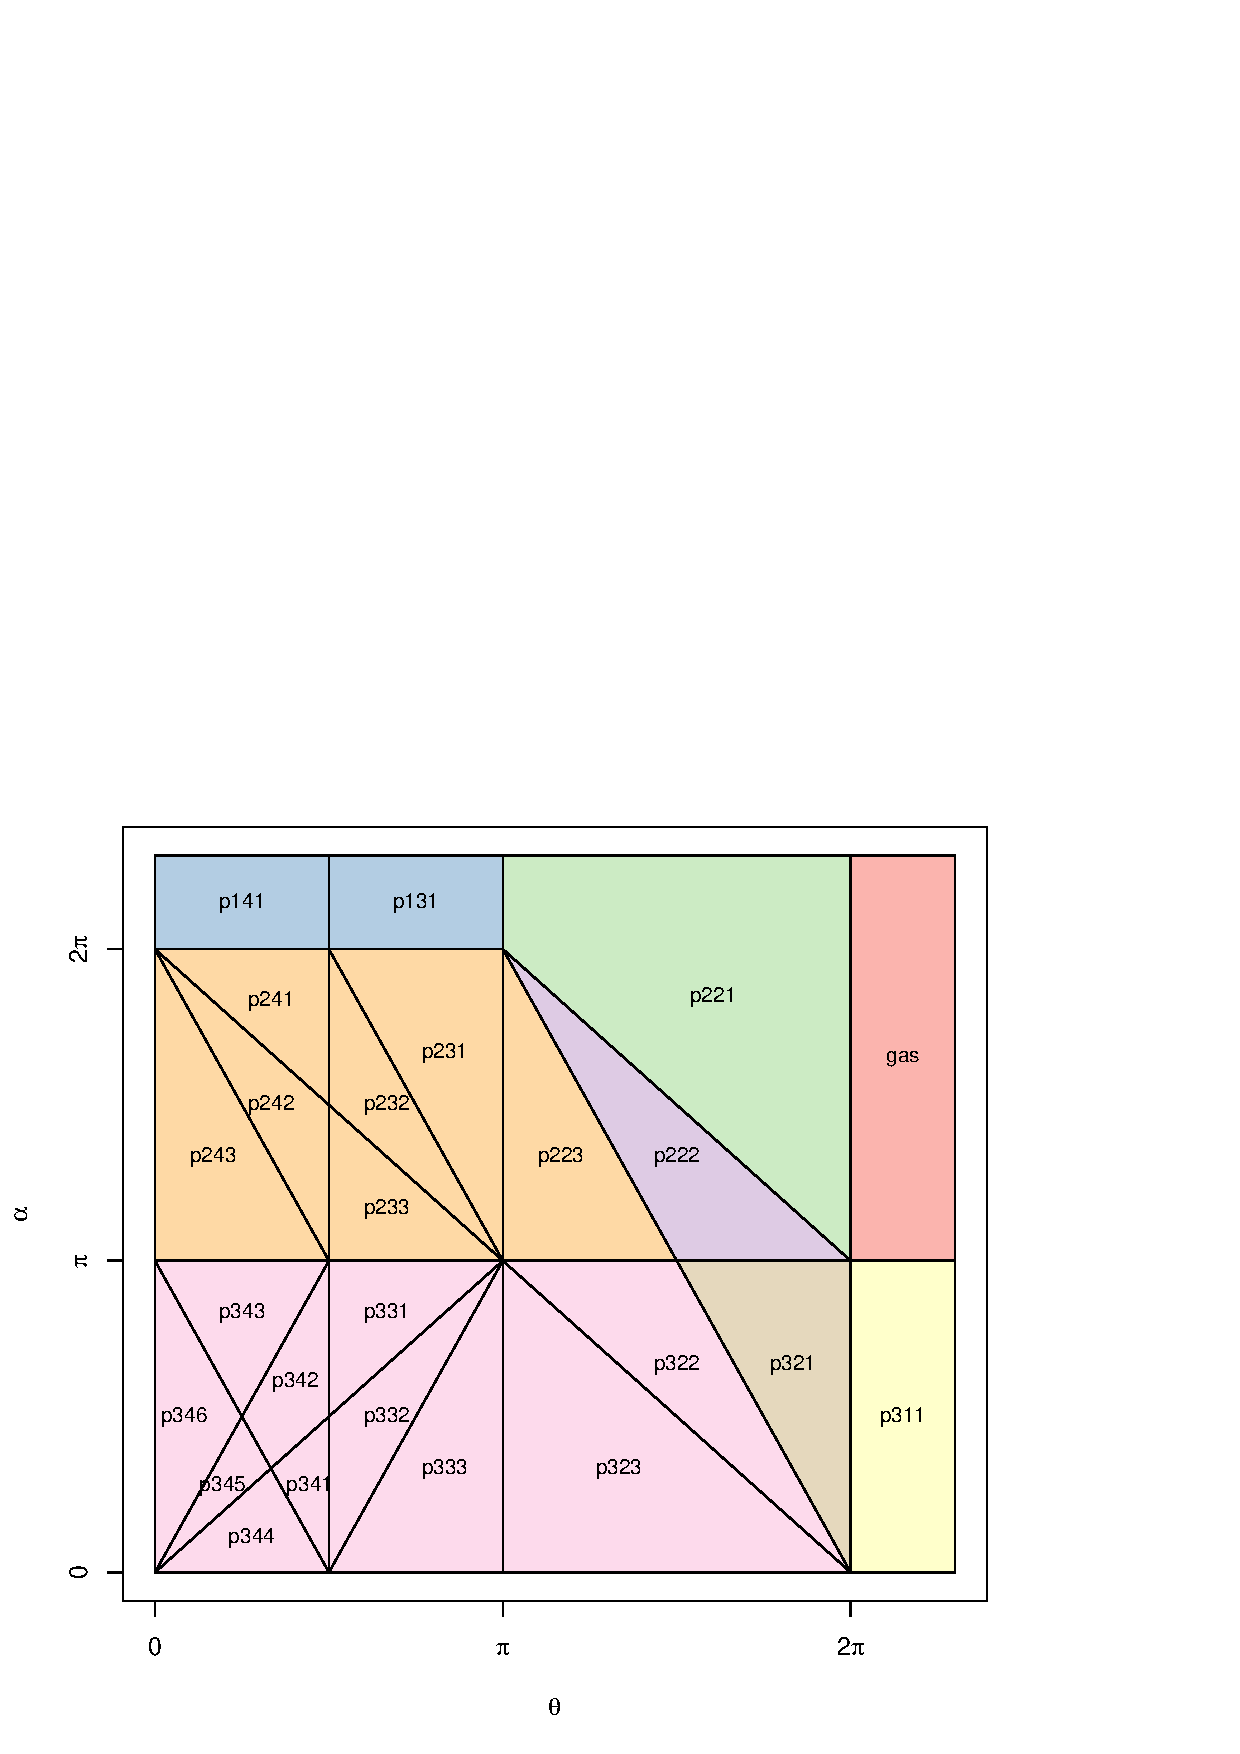
\includegraphics[width=0.6\textwidth]{/home/tim/Dropbox/PhD/Analysis/REM-chapter/imgs/equalRegions.pdf}
\caption[REM Model numbers]{The independently derived models for the whole of parameter space. Regions whose solution for $p$ are equal are coloured similarly. Models are numbered by their row, column and then numbered within that area. The models for $\alpha = 2\pi$ or $\theta =  2\pi$ are shown by extending these regions outside of their real boundaries.}
\label{f:equalRegions}
\end{figure}

\end{comment}

\begin{comment}
\subsection{Contents}
\begin{itemize}
        \item \ref{gas}: {\bf Gas model}
        \item \ref{p311}: {\bf  p311}
        \item \ref{p22}: {\bf  p22}
        \begin{itemize}
                \item \ref{p221}: {\bf  p221}
                \item \ref{p222}: {\bf  p222}
                \item \ref{p223}: {\bf  p223}
        \end{itemize}
        \item \ref{p32}: {\bf  p32}
        \begin{itemize}
                \item \ref{p321}: {\bf  p321}
                \item \ref{p322}: {\bf  p322}
                \item \ref{p323}: {\bf  p323}
        \end{itemize}
        \item \ref{p131}: {\bf  p131}
        \item \ref{p23}: {\bf  p23}
        \begin{itemize}
                \item \ref{p231}: {\bf  p231}
                \item \ref{p232}: {\bf  p232}
                \item \ref{p233}: {\bf p233}
        \end{itemize}
        \item \ref{p33}: {\bf  p33}
        \begin{itemize}
                \item \ref{p331}: {\bf  p331}
                \item \ref{p332}: {\bf  p332}
                \item \ref{p333}: {\bf  p333}
        \end{itemize}
        \item \ref{p141}: {\bf  p141}
        \item \ref{p24}: {\bf  p24}
        \begin{itemize}
                \item \ref{p241}: {\bf  p241}
                \item \ref{p242}: {\bf  p242}
                \item \ref{p243}: {\bf  p243}
        \end{itemize}
        \item \ref{p34}: {\bf  p34}
        \begin{itemize}
                \item \ref{p341}: {\bf  p341}
                \item \ref{p342}: {\bf  p342}
                \item \ref{p343}: {\bf  p343}
        \end{itemize}
\end{itemize}

\end{comment}

%Figure \ref{f:equalRegions} shows the different regions with the upper right being the gas model as derived above and p141 being the model from \citep{rowcliffe2008estimating}. Parameter space is broadly split into three rows ($\alpha \le \pi, \pi \le \alpha < 2\pi$ and $\alpha = 2\pi$) and four columns $(\theta \le \pi/2,  \pi/2 \le \theta \le \pi,  \pi \le \theta < 2\pi$ and $\theta = 2\pi$.) Rows and columns define cells. The equation for $p$ in each region is denoted by three numbers referring to rows, columns and region within that cell (see Fig.~\ref{f:equalRegions}).


\subsection{Gas model} \label{gas}

We assume that animals are in an homogeneous environment, and move in straight lines of random direction with velocity $v$. We allow that our sensor can detect animals at a distance $r$ and that if an animal moves within this detection region they are detected with a probability of 1, independent of distance from the sensor while animals outside the region are never detected.

We then consider movement from the reference frame of the animals so that now, all animals are stationary and randomly distributed in space, while the sensor moves with velocity $v$. If we calculate the area covered by the sensor during the study period we can estimate the number of animals it should encounter. We calculate this as the average width of the sensor region $p$ multiplied by $v$. The average width of the profile is the integral of the profile width over a full circle, divided by $2\pi$. We use $x_i$ to denote the focal angle which is the angle we integrate over. The subscript $i$ distinguishes different angles (see Figure \ref{f:xis}) but here we use $x_1$.  As all models are bilaterally symetric, we can integrate over a half circle, and divide by $\pi$.
\begin{align}
p\text{Gas} =& \frac{1}{\pi}\int\limits_{\frac{\pi}{2}}^{\frac{3\pi}{2}} 2r \; \mathrm{d}x_1\\
p\text{Gas} =& 2r
\end{align}
The number of expected encounters, $z$, for a survey of duration $t$, with an animal density of $D$ is then
\begin{equation}
	z = 2rvtD.
\end{equation}
However, in practice we have the opposite situation. We know the number of encounters and want to estimate the density. We do this be simply rearranging to get
\begin{equation}
	D = z/(2rvt).
\end{equation}
For different values of $\theta$ and $\alpha$, the only thing that changes is that the area covered per unit time is no longer given by $2rv$. Instead of the sensor having a diameter of $2r$, the sensor has a complex diameter that changes with approach angle. The rest of the derivation is just calculating this value for all values of $\alpha$ and $\theta$. However, different regions of this two dimensional parameter space have noncontinuously different models, with different derivations. Therefore we have to identify the regions for which the derivation is the same, and then separately derive $p$ for each region.


\begin{figure}[t]
        \centering
        \begin{subfigure}[t]{0.34\textwidth}
                \centering
                \begin{tikzpicture}[scale=0.39]
                \fullAngleOne{0}{300}{120};
                \end{tikzpicture}
                \caption{$x_1$}
                \label{f:tikz1}
        \end{subfigure}
        ~ 
        \begin{subfigure}[t]{0.22\textwidth}
                \centering
                \begin{tikzpicture}[scale=0.39]
                \fullAngleTwo{0}{80}{75};
                \end{tikzpicture}
                \caption{$x_2$}
                \label{f:x2}
        \end{subfigure}
        ~ 
	\begin{subfigure}[t]{0.22\textwidth}
                \centering
                \begin{tikzpicture}[scale=0.39]
                \fullAngleThree{0}{50}{70};
                \end{tikzpicture}
                \caption{$x_3$}
                \label{f:x3}
        \end{subfigure}%%
	~
	\begin{subfigure}[t]{0.22\textwidth}
                \centering
                \begin{tikzpicture}[scale=0.39]
                \fullAngleFour{0}{80}{70};
                \end{tikzpicture}
                \caption{$x_4$}
                \label{f:x4}
        \end{subfigure}%%
\caption{The location of the focal angles $x_{i\in[1,4]}$. In these figures, the segment shaped detection region is shown in black. The width of this region is shown with a thick red line and a blue rectangle. The direction of animal movement is always downwards, as indicated by the grey arrow.}
\label{f:xis}
\end{figure}



\subsection{Model p311} \label{p311}

p311 is very similar to the gas model except that as $\alpha \le \pi$ the profile width is no longer $2r$ but is instead limited by the width of the animal call. We therefore get a profile width of $2r\sin(\alpha/2)$ instead (see Fig~\ref{f:callExplained}).

\input{/home/tim/Dropbox/PhD/Analysis/REM-chapter/latexFiles/p311.tex}

\subsection{Model p22} \label{p22}

For regions with profiles that are more complex than a circle we need to explicitly write functions for the width of the profile for every approach angle. We then use these functions to find the average profile width for all approach angles by integrating across all $2\pi$ angles of approach and dividing by $2\pi$. 



There are three regions within cell p22. Note that p221 covers the area $\alpha=2\pi$ as well as the triangle below it as these two models are specified exactly the same, rather than happening to have equal results.

These models have up to five regions. 1) The profile width starts, from $x_1=\frac{\pi}{2}$ as $2r$. 2) At $x_1 = \theta/2$, the right hand side of the profile cannot be $r$ wide as the corner of the `blind spot' (see Fig.~\ref{f:blindSpot}) limits its size to being $r\cos(x_1 - \theta/2)$ wide (see Fig.~\ref{f:p22Limit}). 

3) The third profile is only found in p223. If $\alpha < 4\pi - 2\theta$, then at $x_1=\theta/2$, when the profile is perpendicular to the edge of the blind spot, the whole right side of the profile is invisible to the sensor (see Fig.~\ref{f:p223third}). This gives a profile size of just $r$.

4) At some point, the sensor can detect animals once they have passed the blind spot giving a profile width of $r + r\cos(x_1 + \theta/2)$. From $x_1=\pi$, if the animal call is wide enough to be detected in this area, this is the wider profile. This then defines the split between p221 and p222. In p221, with $\alpha > 3\pi - \theta$, the animal call is wide enough that at $x_1=\pi$ the animal can already be detected past the blind spot and so this profile is used. In p222, with $\alpha < 3\pi - \theta$, the latter profile is reached at $5\pi/2 - \theta/2 - \alpha/2$ and is therefore dependant on the sizes of $\alpha$ and $\theta$. 

5) Finally, common to all three models, at $x_1 = 2\pi - \theta/2$ the profile becomes a full $2r$ once again.


\subsubsection{Model p221} \label{p221}

Model p221 exists within the area bounded by $\alpha\le2\pi$, $\theta\le2\pi$ and $\alpha \ge 3\pi - \theta$. It has four regions; it does not include the $r$ profile at $x_1=\pi$. Furthermore, $\theta$ is wide enough that the $r + r\cos(x_1 + \theta/2)$ profile starts at $\pi$. This then gives us


\input{/home/tim/Dropbox/PhD/Analysis/REM-chapter/latexFiles/p221.tex}


\begin{figure}[t]
        \centering
        \begin{subfigure}[t]{0.3\textwidth}
                \centering
                \begin{tikzpicture}[scale=0.38]
        	\sensorOne{220}{120};
       		\directionArrowOne{0}{220}{120};
       		\segmentOne{220}{120};
		\def\angRad{0.6}
		\draw[profile] (0,0) ++  (180 - 120 + 220/2:\angRad) arc (180 - 120 + 220/2: 360 + 180 - 120 - 220/2  :\angRad);
                \end{tikzpicture}
                \caption{Blind spot}
                \label{f:blindSpot}
        \end{subfigure}
~ 
        \begin{subfigure}[t]{0.3\textwidth}
                \centering
                \begin{tikzpicture}[scale=0.38]
                \fullOne{100}{200}{170}
                \end{tikzpicture}
                \caption{Directional Call}
                \label{f:callExplained}
        \end{subfigure}
\caption{A) Shows the area referred to as the `blind spot'. B) For directional calls, with $\alpha<\pi$, the width of the profile can be limited by the call angle or by the detector region.  The detector width is shown in blue, while the call width is shown as a red rectangle. Only where the two overlap, giving a purple area, can an animal be detected. Here we would say the right side of the profile is limited by the sensor, while the left side of the profile is limited by the call angle. The terms in equations would reflect this by containing $\alpha$ if call limited and containing $\theta$ if detector limited.  }
\label{f:p22}
\end{figure}




\subsubsection{Model p222} \label{p222}

Model p222 is bounded by $\alpha \le 3\pi - \theta$, $\alpha \ge 4\pi - 2\theta$ and $\alpha \ge \pi$. It is the same as p221 except that the third profile starts at $5\pi/2 - \theta/2 - \alpha/2$ instead of at $\pi$ which is reflected in the different bounds in the second and third integral.

\input{/home/tim/Dropbox/PhD/Analysis/REM-chapter/latexFiles/p222.tex}

\subsubsection{Model p223} \label{p223}

Model p223 is bound by $\alpha \le 4\pi - 2\theta$, $\alpha \ge \pi$ and $\theta \ge \pi$. It is the same as p222 except that it contains the extra profile with width $r$ (third integral).

\input{/home/tim/Dropbox/PhD/Analysis/REM-chapter/latexFiles/p223.tex}



\begin{figure}[t]
        \centering
        \begin{subfigure}[t]{0.3\textwidth}
                \centering
                \begin{tikzpicture}[scale=0.38]
                \fullAngleOne{0}{220}{160};
                \end{tikzpicture}
                \caption{}
                \label{f:p22Limit}
        \end{subfigure}
        ~ 
        \begin{subfigure}[t]{0.3\textwidth}
                \centering
                \begin{tikzpicture}[scale=0.38]
        	\fill[opacity=\o, sensCol] (0, \lwr) rectangle ({\r}, \upr);       
        	\directionArrowOne{0}{220}{200};
		\draw[profile]     (0,0)  -- (0:\r);
		\fill[ focus]  (180 - 220/2 - 200:\r) ++ (- 220/2 - 220:2*\angRad) arc (- 220/2 - 220:-360-90:2*\angRad) -- (180 - 220/2 - 200:\r) -- cycle;
        	\segmentOne{220}{200};
		\draw  (0,0)  ++(180 - 220/2 - 200:\r) -- ++ (-90: 2);
		\node[left] at (180 - 220/2 - 200:\r) {$\frac{\alpha}{2}$};
                \end{tikzpicture}
                \caption{}
                \label{f:p223third}
        \end{subfigure}
        ~ 
        \begin{subfigure}[t]{0.3\textwidth}
                \centering
                \begin{tikzpicture}[scale=0.38]
                \fullOne{0}{220}{240};
		\fill[ focus]  (180 - 220/2 - 240:\r) ++ (- 220/2 - 220:2*\angRad) arc (- 220/2 - 220:-360-90:2*\angRad) -- (180 - 220/2 - 240:\r) -- cycle;
        	\segmentOne{220}{240};
		\node[left] at (180 - 220/2 - 240:\r) {$\frac{\alpha}{2}$};
                \end{tikzpicture}
                \caption{}
                \label{f:p223fourth}
        \end{subfigure}
\caption{A) The second integral in p22 with width $r + r\cos(x_1 - \theta/2)$ B) The third integral in p223. The angle shown in red is $\alpha/2$. As it is small, animals to the right of the detector cannot be detected. C) After further rotation, $\alpha/2$ is now bigger than the angle shown and animals to the right of the detector can again be sensed.   }
\label{f:p22}
\end{figure}


\subsection{Model p32} \label{p32}

Cell p32 contains three regions that differ in ways reminiscent of the models in p22. There are four possible profile widths. 1) As $\alpha$ is less than $\pi$ the profile is smaller than $2r$, even when the sensor width is a full diameter. When this is the case, the profile width is instead $2r\sin(\alpha/2$. 2) Similar to p22, at a certain point the blind spot of the sensor area limits the profile width (see Fig.~\ref{f:p32AT}). This gives a profile width of $r\sin(\alpha/2) + r\cos(x_1 - \theta/2)$. 3) Also similar to p22, there can be a point where the right side of the profile is 0 giving a profile width of $r\sin(\alpha/2)$. 4) If $\alpha \le 2\pi - \theta$, then at $\theta/2 + \pi/2 + \alpha/2 $ the profile width become 0 (see Fig.~\ref{f:p32Last}). This inequality distinguishes between p322 and p323. The profile $r\sin(\alpha/2)$ starts at $\theta/2 + \pi/2$ while at $5\pi/2 - \alpha/2 - \theta/2$ the profile returns to size $2r\sin(\alpha/2)$. If $\theta/2 + \pi/2 \ge 5\pi/2 - \alpha/2 - \theta/2$ we go straight into the  $2r\sin(\alpha/2)$ profile and miss the $r\sin(\alpha/2)$ profile.  p321 and p322 are seperated by this inequality which simplifies to $\alpha \le 4\pi - 2\theta$. 



\begin{figure}[t]
        \centering
        \begin{subfigure}[t]{0.3\textwidth}
                \centering
                \begin{tikzpicture}[scale=0.38]
                \fullOne{100}{200}{170}
                \end{tikzpicture}
                \caption{}
                \label{f:p32AT}
        \end{subfigure}
~ 
        \begin{subfigure}[t]{0.3\textwidth}
                \centering
                \begin{tikzpicture}[scale=0.38]
                \fullOne{0}{220}{330}; % 220/2 + 90 +130
                \end{tikzpicture}
                \caption{}
                \label{f:p32Last}
        \end{subfigure}
\caption{A) The third integral in p32. The right side of the profile is limited by the size of the sensor region (blue region) while the left side of the profile is limited by the size of the call angle (red region). The profile width is the purple region where these two overlap. B)     }
\label{f:p32}
\end{figure}

\subsubsection{Model p321} \label{p321}

p321 is bounded by $\alpha \ge 4\pi - 2\theta$, $\alpha \le \pi$ and $\theta \le 2\pi$. As $\alpha \ge 4\pi - 2\theta$, there is no $r\sin(\alpha/2)$ profile. As $\alpha \le 4\pi - 2\theta$, the profile returns to $2r\sin(\alpha/2)$ rather than going to 0.

\input{/home/tim/Dropbox/PhD/Analysis/REM-chapter/latexFiles/p321.tex}

\subsubsection{Model p322} \label{p322}

p322 is bounded by $4\pi - 2\theta \le \alpha \le 4\pi - 2\theta$ and $\alpha \le \pi$. Therefore there is a $r\sin(\alpha/2)$ profile but no $0r$ profile.

\input{/home/tim/Dropbox/PhD/Analysis/REM-chapter/latexFiles/p322.tex}

\subsubsection{Model p323} \label{p323}

Finally p323 is bounded by  $\alpha \le 4\pi - 2\theta $, $\alpha\le\pi$ and $\theta \le \pi$. It is the same as p322 except that the profile becomes $2r$ rather than returning to $2r\sin(\alpha/2)$.

\input{/home/tim/Dropbox/PhD/Analysis/REM-chapter/latexFiles/p323.tex}


\begin{figure}[t]
        \centering
        \begin{subfigure}[t]{0.3\textwidth}
                \centering
                \begin{tikzpicture}[scale=0.38]
                \fullAngleFour{0}{140}{30}
		
                \end{tikzpicture}
                \caption{}
                \label{f:p131AT}
        \end{subfigure}
~ 
        \begin{subfigure}[t]{0.3\textwidth}
                \centering
                \begin{tikzpicture}[scale=0.38]
                \fullAngleFour{0}{130}{110};
                \end{tikzpicture}
                \caption{}
                \label{f:p131behindFull}
        \end{subfigure}
\caption{A) and B) The third and fourth profiles of p131. The left side of of both profiles is of width $r$ while the right side is $- r\cos(x_4 - \theta)$ and $- r\cos(x_4)$ respectively. }
\label{f:p131}
\end{figure}

\subsection{Model p131} \label{p131}

p131 is the first model with $\theta < \pi$. Whereas previously the focal angle has always been $x_1$, we now use different focal angles. $x_2$ and $x_3$ correspond to $\gamma_1$ and $\gamma_2$ in \cite{rowcliffe2008estimating} while $x_4$ is new. They are described in Fig.~\ref{f:xis}. 

There are five different profiles in p131. 1) $x_2$ has an interval of $[\pi/2, \theta/2]$ which is from the angle of approach being directly towards the sensor until the profile is parellel to the left hand radius of the sensor segment. During this region the profile width is $2r\sin\left(\theta/2\right)\sin(x_2)$ which is calculated using the equation for the length of a chord (see Fig.~\ref{f:x2}). Note that while rotating anti-clockwise (as usual) $x_2$ decreases in size. 2) From here, we examine focal angle $x_4$ (note that $x_3$ is used in later models, but is not relevant here.)  The left side of the profile is a full radius while the right side is limited to $- r\cos(x_4 - \theta)$ (see Fig.~\ref{f:p131AT}). 3) At $x_4 =  \theta - \pi/2$, the profile is perpendicular to the edge of the sensor area. Here, the right side of the profile is $0r$. 4) When $x_4 = \pi/2$ the angle of approach is from behind the sensor, but we can once again be detected on the right side of the sensor (see Fig.~\ref{f:p131behindFull}). Therefore the width of the profile is $r - r\cos(x_4)$. 5) Finally, we enter the $x_2$ region, but from behind. 

\input{/home/tim/Dropbox/PhD/Analysis/REM-chapter/latexFiles/p131.tex}

\subsection{Model p23} \label{p23}

The models in cell p23 have the five potential profiles in p131 but not all profiles occur in each model, and the angle at which transitions occur are different. Furthermore, there is one extra profile possible. When approaching the sensor from behind, there is a period where the profile is $r$ wide as in p131. At some point the right side of the profile becomes viable again. If this occurs in the $x_4$ region, the profile width becomes  $r - r\cos(x_4)$ as in p131. However, as $\alpha$ is now less than $2\pi$, the right side of the profile might not be viable until we are in the second $x_2$ region. In this case, when we first enter the second $x_2$ region, the profile has a width of $r\cos(x_2 - \theta/2)$. This occurs only if $\alpha \le 3\pi - 2\theta$. This is inequality is found by noting that the right side of the profile become viable at $x_4 = 3\pi/2 - \alpha$ but the $x_2$ region starts at $x_4 = \theta$. The new profile in $x_2$ will only occur if  $ \theta < 3\pi/2 - \alpha/2$ which is rearranged to find the inequality above. This defines the boundary between p231 and p232.

As $\alpha \le 2\pi$ it is possible that when the angle of approach is from directly behind the sensor the animal will not be detected at all. This is the case if $\alpha/2\le \pi-\theta/2$ as shown in Fig.~\ref{f:p23behind}. This inequality defines the boundary between p232 and p233.

\begin{figure}[t]
        \centering
        \begin{subfigure}[t]{0.4\textwidth}
                \centering
                \begin{tikzpicture}[scale=0.38]
		\sensorTwo{120}{270};
		\directionArrowTwo{0}{120}{270};
		\fill[ focus]  (180 + 90 - 120/2:\r) ++ (+ 90 - 150/2:2*\angRad) arc (+ 90 - 150/2:-90:2*\angRad) -- (180 + 90 - 120/2:\r) -- cycle;
		\segmentTwo{120}{270};
		\node[left] at (180 + 90 - 120/2:\r) {$\frac{\alpha}{2}$};
                \end{tikzpicture}
                \caption{}
                \label{f:p23behind}
        \end{subfigure}

\caption{A) If $\alpha/2$, shown in green, is less than $\pi - \theta/2$, as is the case here, then the width of the profile when an animal approaches directly from behind is zero. }
\label{f:p23}
\end{figure}


\subsubsection{Model p231} \label{p231}

p231 is bounded by $\alpha \ge 3\pi - 2\theta$, $\alpha \le 2\pi$ and $\theta\le\pi$.

p231 has all five profiles as found in p131. However, the change from the $r$ profile (third integral) to the $r - r\cos(x_4)$ profile (fourth integral) occurs at $x_4 = 3\pi/2 - \alpha/2$ instead of at $x_4 = \theta$. 

\input{/home/tim/Dropbox/PhD/Analysis/REM-chapter/latexFiles/p231.tex}


\subsubsection{Model p232} \label{p232}

p232 is bounded by $\alpha \le 3\pi - 2\theta$, $\alpha\ge 2\pi-\theta$ and $\theta\le\pi$.

p232 does not have the fourth integral from p231 as the right side of the profile does not become viable until after the $x_4$ region has ended and the $x_2$ region has begun. Therefore the second $x_4$ integral has an upper limit of $\theta $ and the integral after has a width of $r\cos(x_2 - \theta/2)$ and is integrated with respect to $x_2$. The final integral starts at $x_4 = 3\pi/2 - \alpha/2 - \theta/2$ and has the full width of $2r\sin(x_2)\sin(\theta/2)$.

\input{/home/tim/Dropbox/PhD/Analysis/REM-chapter/latexFiles/p232.tex}

\subsubsection{Model p233} \label{p233}

Finally, p233 is bounded by $\alpha\le \pi$, $\theta\ge \pi/2$ and $\alpha \le 3\pi - 2\theta$. p233 is the same as p232 except that the final profile width is zero and this profile is reached at $\alpha/2+\theta/2-\pi/2$. 

\input{/home/tim/Dropbox/PhD/Analysis/REM-chapter/latexFiles/p233.tex}

\subsection{Model p33} \label{p33}
 
The models in p33 are described with the two focal angles used in models p23, $x_2$ and $x_4$. As $\alpha \le\pi$ an animal can never be detected if it is approaching the detector from behind. This makes these models simpler in that they go through the $x_2$ and $x_4$ eons only once each. 

There are five potential profile sizes. At the beginning of $x_2$, with an approach direction directly towards the sensor, the factor that limits the width of the profile can either be 1) the sensor width,  in which case the profile width is $2r\sin\left(\theta/2\right)\sin(x_2)$, or 2) the call width, in which case the profile width is instead $2r\sin(\alpha /2)$ (see Figure~\ref{f:p33})

\begin{figure}[t]
        \centering
        \begin{subfigure}[t]{0.4\textwidth}
                \centering
                \begin{tikzpicture}[scale=0.38]
		\fullTwo{170}{100}{80};
                \end{tikzpicture}
                \caption{}
                \label{f:p33x2a}
        \end{subfigure}
	~
	\begin{subfigure}[t]{0.4\textwidth}
                \centering
                \begin{tikzpicture}[scale=0.38]
		\fullTwo{40}{100}{80};
                \end{tikzpicture}
                \caption{}
                \label{f:p33x2t}
        \end{subfigure}

\caption{A) As $\alpha > \theta$ the profile width (purple) is limited by the sensor region, not the call angle (red). The profile width is $2r\sin\left(\frac{\theta}{2}\right)\sin(x_2)$. B) As $\alpha < \theta$ the profile width is limited by the call angle rather than the sensor region (blue). The profile width is $2r\sin\left(\frac{\alpha}{2}\right)$   }
\label{f:p33}
\end{figure}

3) The next potential profile in $x_2$ has a width of $r\sin(\alpha/2) - r\cos(x_2 + \theta/2)$ as the right side of the profile is limited by the width of the sensor region while the left side is limited by the call width. However, the angle at which the profile starts depends on whether the first profile was 1) or 2) above. If the first profile is profile 1) then the profile is limited on both sides by the sensor region and then the left side of the profile becomes limited by the call width. This happens at $x_2 = \pi/2 - \alpha/2 + \theta/2$. If however the first profile was 2) then the first profile is limited by the call width. We move into the new profile when the right side of the profile becomes limited by the sensor region. This occurs at $x_2 = \pi/2 + \alpha/2 - \theta/2$.


In the $x_4$ region the left side of the profile is always $r\sin(\alpha /2)$ while the right side is either 4) 0, giving a profile of $r\sin(\alpha /2)$, or 5) limited by the sensor giving a profile of size $r\sin (\alpha /2) -r\cos(x_4-\theta) $.

\subsubsection{Model p331} \label{p331}

p331 is bounded by $\alpha \ge \theta$, $\alpha \le\pi$ and $\theta \le \pi$.

As $\alpha $ is large the first profile is limited by the size of the sensor region giving it a width of $2r\sin\left(\theta/2\right)\sin(x_2)$. It is the only one of the three p33 models to start in this way. Later on, still with $x_2$ as the focal angle the left side of the profile does become limited by the call width. So at $x_2= \pi/2 - \alpha/2 + \theta/2$ the profile width becomes $r\sin(\alpha/2) - r\cos(x_2 + \theta/2)$. 

As we enter the $x_4$ region, the profile remains limited by the call on the left and by the sensor on the right, giving a profile width of  $r\sin (\alpha /2) -r\cos(x_4-\theta) $. Finally, at $x_4 = \theta - \pi/2$ the right side of the profile becomes zero and the profile is width is $r\sin(\alpha /2)$.

\input{/home/tim/Dropbox/PhD/Analysis/REM-chapter/latexFiles/p331.tex}

\subsubsection{Model p332} \label{p332}

p332 is bounded by $\theta \ge \pi/2$, $\alpha \le \theta$ and $\alpha \ge 2\theta -\pi$.

p332 is largely similar to p331. However, as $\alpha \le \theta$ the first profile is limited by $\alpha$ and not by the detection region. Therefore the first profile has width $2r\sin(\alpha /2)$. This also means the transition to the second profile occurs at  $x_2 = \pi/2 + \alpha/2 - \theta/2$ instead of  $x_2 = \pi/2 - \alpha/2 + \theta/2$.

\input{/home/tim/Dropbox/PhD/Analysis/REM-chapter/latexFiles/p332.tex}



\subsubsection{Model p333} \label{p333}

p333 is bounded by $\alpha \le 2\theta -\pi$ and $\theta \le \pi$.

p333 is similar to p332 except that the profile does not become limited by sensor at all during the the $x_4$ regions. Therefore, at $x_4 = 0 $ the profile is still of width $2r\sin(\alpha /2)$. Only at $x_4 = \theta - \pi/2 - \alpha/2$ does the profile become limited on the right by the sensor region.

\input{/home/tim/Dropbox/PhD/Analysis/REM-chapter/latexFiles/p333.tex}

\subsection{Model p141} \label{p141}

p141 is the model from \citep{rowcliffe2008estimating}. It has $\alpha =2\pi$ and $\theta \le \pi/2$. It has three profile widths, two of which are repeated, once as the animal approaches from on front of the sensor and once as the animal approaches from behind the sensor.

Starting with an approach direction of directly towards the sensor, and examining focal angle $x_2$, the profile width is $2r\sin(x_2)\sin(\theta/2)$. When the profile is perpendicular to the radius edge of the segment sensor region, we instead examine $x_3$ where the profile width is $r\sin(x_3)$. At $x_3=\pi/2$ the profile becomes simply $r$ and this continues for $\theta $ radians of $x_4$. Finally the $x_3$ and $x_2$ are repeated with an approach direction from behind the sensor. 

\input{/home/tim/Dropbox/PhD/Analysis/REM-chapter/latexFiles/p141.tex}

\subsection{Model p24} \label{p24}

In the models in p24, the sensor has $\theta \le pi/2$ as in p141. As $\alpha \ge \pi/2$ a lot of the profiles are similar to p141. Specifically, the first three profiles are always the same as the first three profiles of p141. This is because when an animal is moving towards the sensor, the $\alpha \ge \pi$ call is no different to a $2\pi$ call. However, when approaching the sensor from behind, things are slightly different. The animal can only be detected by the sensor if it's call is wide enough that it can be detected once it has passed the sensor. 

The second $x_3$ profile is always the same width as in p141. This is because there is no detection region to one side of the sensor so this side is unaffected by call width, while the width of the other side of the profile is unaffected by $\alpha$ as when $\alpha>\pi$ the profile width will never be limited by $\alpha$. If $\alpha \le 2\pi + 2\theta$, the animal becomes undetectable during this profile when  $x_3$ has decreased in size to $\pi - \alpha/2$. This inequality marks the boundary between p243 and p242. 

As the focal angle moves from $x_3$ to $x_2$  at $x_3=\theta$, we can see that if $\alpha \ge 2\pi + 2\theta$, then the $x_2$ region is reached before the animal become undetectable. When this second $x_2$ region is reached, the profile starts with width $r\cos(x_2 - \theta/2)$ as at the beginning of the $x_2$ profile as only animals approaching to the left of the sensor are detectable. The sensor is directly behind the right side of the profile.

During this second $x_2$ profile the call angle needed for animals to be detected to the left of the detector is increasing while the angle needed for animals to be detected to the right of the detector is decreasing. Therefore, either the left side becomes undetectable, making both sides undetectable (this occurs if $\alpha \le 2\pi - \theta$ as in p242) or the right becomes detectable (if $\alpha \ge 2\pi - \theta$ as in p241), making both sides detectable and giving a profile width of $2r\sin(x_2)\sin(\theta/2)$.


\subsubsection{Model p241} \label{p241}

p241 is bounded by $\alpha \ge 2\pi - \theta$, $\alpha \le 2\pi$ and $\theta \le \pi/2$.

It is the same as p141 except that it includes the extra profile in $x_2$ (the fifth integral) where only animals approaching to the left of the profile are detected.

\input{/home/tim/Dropbox/PhD/Analysis/REM-chapter/latexFiles/p241.tex}

\subsubsection{Model p242} \label{p242}

p242 is bounded by $\alpha \le 2\pi - \theta$, $\alpha \ge 2\pi + 2\theta$ and $\theta \le \pi/2$

p242 is the same p241 except that as $\alpha \le 2\pi - \theta$, animals that approach from directly behind the detector are not detected. Therefore at $x_2 = \alpha/2 + \theta/2 - \pi/2$ the profile width goes to zero and therefore the last integral in p241 is not included.

\input{/home/tim/Dropbox/PhD/Analysis/REM-chapter/latexFiles/p242.tex}



\subsubsection{Model p243} \label{p243}

p243 is bounded by $\alpha \ge 2\pi + 2\theta$, $\alpha \ge \pi$ and $\theta \ge 0$.

It is similar to p242 but doesn't include the last integral as during the $x_3$ profile, at $x_3 = \pi - \alpha/2$ the call width is too small for any animals to be detected, so the profile width goes to zero.

\input{/home/tim/Dropbox/PhD/Analysis/REM-chapter/latexFiles/p243.tex}





\subsection{Model p34} \label{p34}

Cell p34 is split into six models rather than three like most of the other cells. As $\alpha < \pi$, animals approaching the sensor from behind can never be detected, so unlike p141, the second $x_2$ and $x_3$ profiles are always zero. The six models are split by three inequalities that relate to the models as follows.

\begin{figure}[t]
        \centering

        \begin{subfigure}[t]{0.4\textwidth}
                \centering
                \begin{tikzpicture}[scale=0.38]
                \fullFour{0}{40}{0};
		\fill[ focus] (40:3*\angRad) -- ++  (-90:3.5*\angRad) arc (-90:-90-40:3.5*\angRad) --cycle;
		\draw (40:3*\angRad) -- ++  (-90:5*\angRad) node[ left] {$\frac{\alpha}{2}$};
		%\segmentOne{220}{240};
		%\node[left] at (180 - 220/2 - 240:\r) {$\frac{\alpha}{2}$};
                \end{tikzpicture}
                \caption{$x_4=0$}
                \label{f:p34nox4}
        \end{subfigure}
	~
        \begin{subfigure}[t]{0.4\textwidth}
                \centering
                \begin{tikzpicture}[scale=0.38]
		\fullTwo{50}{80}{65};
                \end{tikzpicture}
                \caption{}
                \label{f:p34taprof}
        \end{subfigure}
        
\caption{A) At $x_4 = 0$, if $\alpha < \pi - 2\theta$ then $\alpha/2$ is too small for an animal to be detected at all during the $x_4$ profile. B) The left of the profile is limited by the call width, not the sensor (blue). On the right, the profile is limited by the sensor and not the call (red). Overall the profile width is $r\sin(\alpha/2) - r\cos(x_2 + \theta/2)$.     }
\label{f:p34}
\end{figure}

Models with $\alpha \le \pi - 2\theta$  have no $x_4$ profile. This is because at $x_4 = 0$, the call angle is already too small to be detected as can be seen in Figure~\ref{f:p34nox4} where $\alpha/2 < \pi/2 - \theta$ which simplifies to give the previous inequality.

Models with $\alpha \le \theta$ are limited by $\alpha$ in the first, $x_2$ region (see Figure~\ref{f:p33}), rather than being limited by $\theta$. Therefore this first profile is of width $2r\sin(\alpha/2)$ rather than $2r\sin(\theta/2)\sin(x_2)$.

Finally, models with $\alpha \le 2\theta$ have a second profile in $x_2$ where to one side of the sensor $\alpha$ is the limiting factor of profile width, while on the other side $\theta$ is (see Figure~\ref{f:p34taprof}). This gives a width of $r\sin(\alpha/2) - r\cos(x_2 + \theta/2)$. This profile doesn't occur in models with $\alpha \ge 2\theta$.

\subsubsection{Model p341} \label{p341}

p341 is bounded by $\alpha \le \theta$, $\alpha \ge \pi - 2\theta$ and $\theta \le \pi/2$. Therefore it does contain a $x_4$ profile, starts with an $\alpha$ limited profile and does contain the $r\sin(\alpha/2) - r\cos(x_2 + \theta/2)$ profile in $x_2$.

\input{/home/tim/Dropbox/PhD/Analysis/REM-chapter/latexFiles/p341.tex}

\subsubsection{Model p342} \label{p342}

p342 is the only model with a tetrahedral bounding region. It is bounded by $\alpha \ge \theta$, $\alpha \ge \pi - 2\theta$, $\alpha \le 2\theta$ and $\theta \le \pi/2$. Therefore it does contain a $x_4$ profile, but starts with a $\theta$ limited profile. It does contain the $r\sin(\alpha/2) - r\cos(x_2 + \theta/2)$ profile in $x_2$.

\input{/home/tim/Dropbox/PhD/Analysis/REM-chapter/latexFiles/p342.tex}

\subsubsection{Model p343} \label{p343}

p343 is bounded by $\alpha \ge \pi - 2\theta$,  $\alpha \ge 2\theta$ and $\alpha \le \pi$. It starts with a $\theta$ limeted profile and has a $x_4$ profile. However, it does not contain the $r\sin(\alpha/2) - r\cos(x_2 + \theta/2)$ profile.

\input{/home/tim/Dropbox/PhD/Analysis/REM-chapter/latexFiles/p343.tex}


\subsubsection{Model p344} \label{p344}

p344 is bounded by $\alpha \le \pi - 2\theta$, $\alpha \le \theta$ and $\alpha < 0$. Therefore it does not contain a $x_4$ profile. It starts with an $\alpha$ limited profile and contains the $r\sin(\alpha/2) - r\cos(x_2 + \theta/2)$ profile in $x_2$.


\input{/home/tim/Dropbox/PhD/Analysis/REM-chapter/latexFiles/p344.tex}

\subsubsection{Model p345} \label{p345}

p345 is bounded by $\alpha \le \pi - 2\theta$, $\alpha \ge \theta$ and $alpha \le 2\theta$. It starts with a $\theta$ limited profile. It does contain the $r\sin(\alpha/2) - r\cos(x_2 + \theta/2)$ profile in $x_2$ but does not have a $x_4$ profile.

\input{/home/tim/Dropbox/PhD/Analysis/REM-chapter/latexFiles/p345.tex}

\begin{comment}
\begin{figure}[t]
\centering
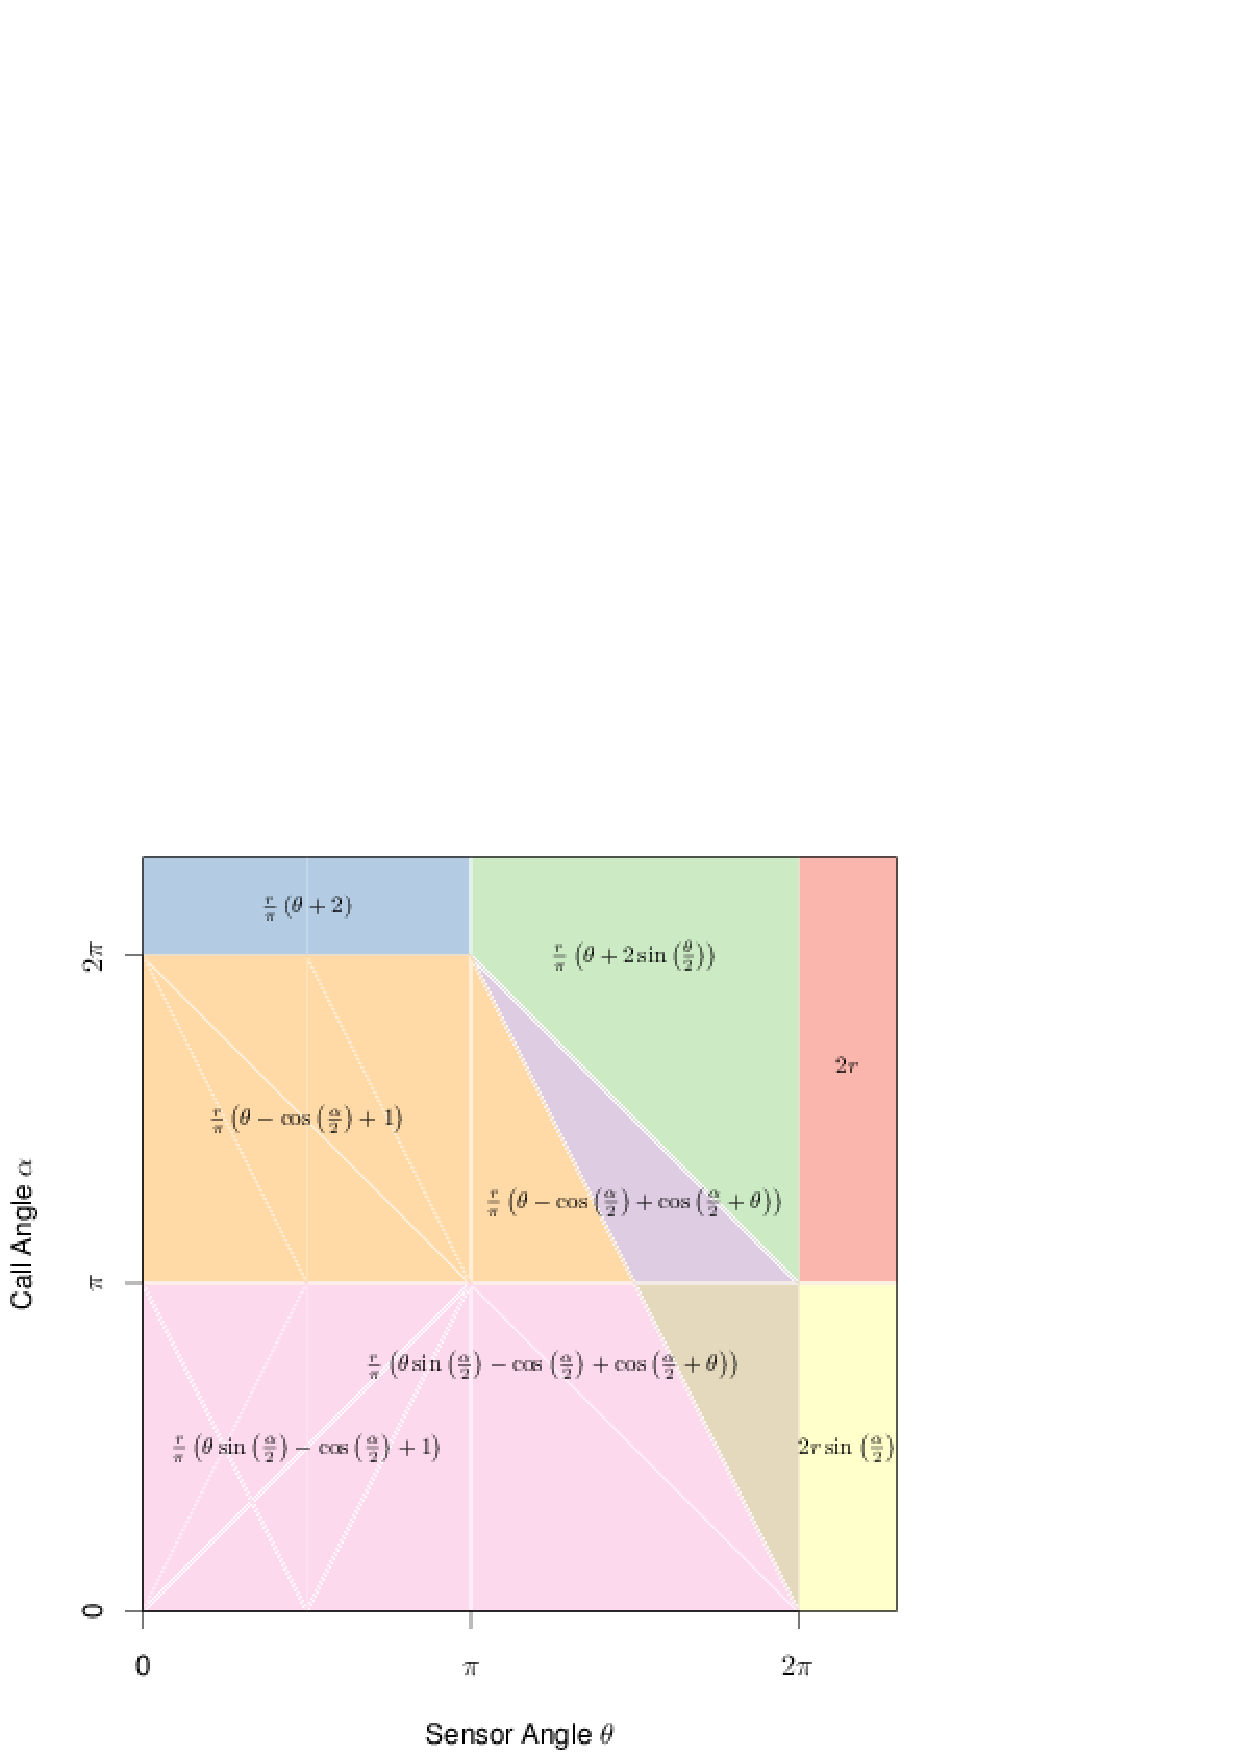
\includegraphics[width=1\textwidth]{/home/tim/Dropbox/PhD/Analysis/REM-chapter/imgs/equalModelResults.pdf}
\caption[REM model solutions]{The results of the models grouped so that all the regions with equal results are presented only once.}
\label{f:equalModelResults}
\end{figure}
\end{comment}

\subsubsection{Model p346} \label{p346}

Finally, p346, the last model, is bounded by y $\alpha \le \pi - 2\theta$, $alpha \ge 2\theta$ and $\theta \ge 0$. Therefore it starts with a $\theta$ limited profile. However it doesn't contain the extra $x_2$ profile nor a $x_4$ profile.

\input{/home/tim/Dropbox/PhD/Analysis/REM-chapter/latexFiles/p346.tex}









\clearpage
\bibliographystyle{../mee.bst}	
\bibliography{../lucas-moorcroft-etal-refs.bib}	

\end{document}


